\emph{Algebraisch:} Die Orte der beiden Fahrzeuge sind
\begin{align}
 s_1 &= v\,t, \qquad s_2 = \frac{1}{2}a\,t^2
\end{align}
Sie treffen sich, wenn $s_1 = s_2$ ist. Ausser der Lösung $t = 0$ (Start) folgt aus $v = \frac{1}{2}a\,t$
\begin{align}
 t &= \tFF = \frac{2\cdot\vF}{\aF} = \tF \approx \result{\tFP{0}{2}}
\end{align}
Die Fahrzeuge haben dann die Strecke
\begin{align}
 s &= v\,t = \sFF = \frac{2\cdot\left(\vF\right)^2}{\aF} = \sF \approx \result{\sFP{0}{2}}
\end{align}
zurückgelegt.

\emph{Graphisch:} Im $s(t)$-Diagramm ist das erste Fahrzeug eine Gerade durch den Ursprung, das zweite eine Parabel mit waagrechter Tangente im Ursprung. Der zweite Schnittpunkt ist das Treffen.

\begin{center}
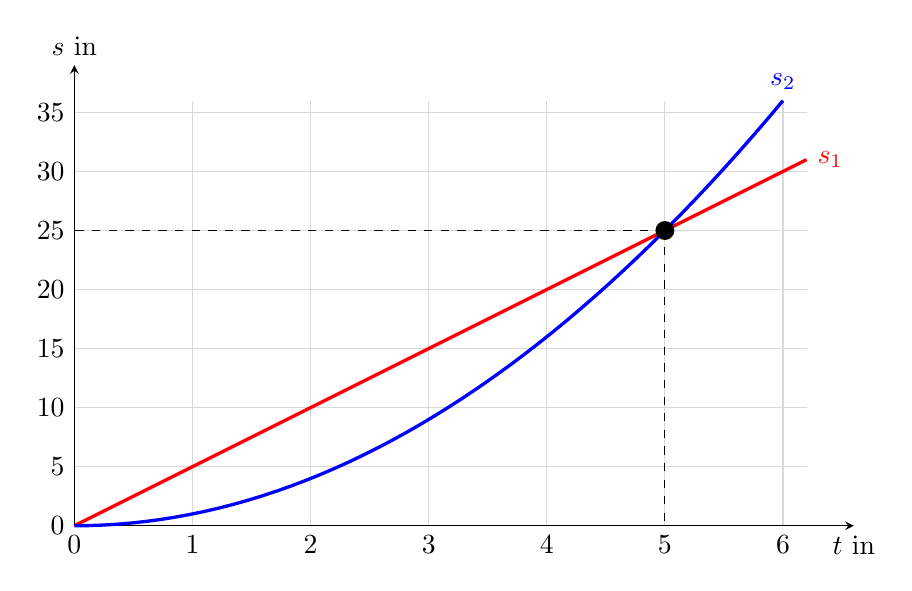
\begin{tikzpicture}[>=stealth, xscale=1.5, yscale=0.15]
 \foreach \x in {1,...,6} \draw[gray!30] (\x,0) -- (\x,36);
 \foreach \y in {5,10,...,35} \draw[gray!30] (0,\y) -- (6.2,\y);
 \draw[->] (0,0) -- (6.6,0) node[below] {$t$ in \si{\second}};
 \draw[->] (0,0) -- (0,39) node[above] {$s$ in \si{\meter}};
 \foreach \x in {0,...,6} \node[below] at (\x,0) {\x};
 \foreach \y in {0,5,...,35} \node[left] at (0,\y) {\y};
 \draw[red, very thick] (0,0) -- (6.2,31) node[right] {$s_1$};
 \draw[blue, very thick, domain=0:6, samples=50] plot (\x, {\x*\x}) node[above] {$s_2$};
 \fill (5,25) ellipse (0.08 and 0.8);
 \draw[dashed] (5,25) -- (5,0);
 \draw[dashed] (5,25) -- (0,25);
\end{tikzpicture}
\end{center}
